%************************************************
\chapter{Evaluation Scenarios}\label{ch:evaluation_scenarios}
%************************************************
In this chapter we detail the scenarios we have imagined for our test subjects to guide them in evaluating the EgoSim framework. The first scenario has the purpose of making the user familiar with the framework. The second scenario was imagined for the simulation user role, where the subject is evaluating a simulation built using our framework. In the third scenario we have imagined a problem which a system designer can solve using the EgoSim framework.\\

We have built the first two prototypes into executable binaries for three major operating systems: Mac OS X, Windows and Linux. The builds are included with the thesis in the \emph{EvaluationPrototypes.zip} archive. They are also available at \url{http://karolyszanto.ro/MastersThesis/evaluation/prototypes/}.

Videos of running the three scenarios are available; see Appendix \ref{ch:videos}.\\

%************************************************
\section{Scenario 1: WarmupTask} % (fold)
\label{sec:eval_warmup_scenario}
%************************************************
This first scenario is meant to make you familiar with the simulator's concepts and interactions. The environment is made up by two tables; the first table has two items on it: a pen and a small statue. The other table is empty. All entities in this scenario can be interacted with. A screenshot of the running simulation is depicted in Figure \ref{fig:eval_warump}.\\

A recording of the running scenario is available; see Appendix \ref{ch:videos}.\\

\begin{figure}[H]
	\centering
	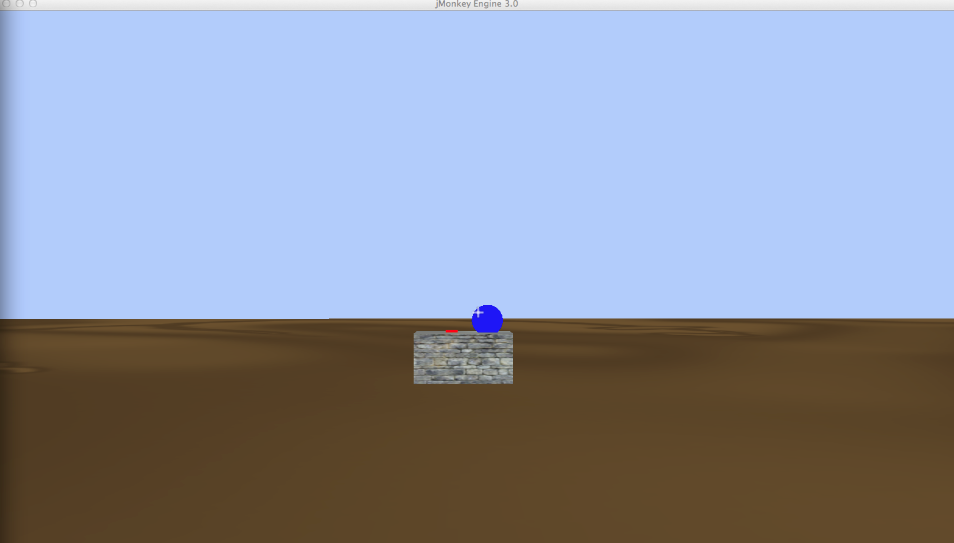
\includegraphics[width=0.8\linewidth]{gfx/Chapter_EvaluationScenarios/prototype1}
	\caption{Sceenshot of the running Warm-up simulation}
	\label{fig:eval_warump}
\end{figure}

Your task is to walk around and interact with the environment while observing the SSM spaces in the ContextClient. N.B.: The client is automatically refreshed every second. As part of the actions you carry out, please try out the followings:
\begin{enumerate}
	\item Move far away from the first table (facing the table), until in the perception space contains only Table1 (it might contain Table2 as well if it's in your visual range). Slowly move towards Table1. At certain distances the PerceptionSpace, RecognizableSet and ExaminableSet will be populated.
	\item Try interacting with the pen while it IS NOT part of the ActionSpace. You are informed that the agent is too far.
	\item Try interacting with the pen while it IS part of the ActionSpace. The pen gets picked up.
	\item Move with the pen towards Table2. While Table2 IS NOT in the ActionSpace, try to interact with it. You are informed that the agent is too far.
	\item While Table2 IS in the ActionSpace and with the pen picked up, try to interact with the table. Table2 is a surfaces and the pen can be placed onto it.
	\item While not holding anything in your hands and while Table2 IS in the ActionSpace, try to it up. Table2 is too heavy for the agent carry.
	\item Move towards the Statue until it's in the ActionSpace and try to interact with it. Interacting with the Statue requires a different implementation than the standard piking up object which is not implemented in this iteration.
	\item Pick up the pen. With the pen picked up and the statue in the ActionSpace, try to interact with the Statue. You can't, because Statue is not a surface. Future releases will handled this more complex scenario as well.
\end{enumerate}

When you arrive to this point, you have successfully performed the WarmUp Task.
% section eval_warmup_scenario (end)
%************************************************
\section{Scenario 2: Assisted Living Facility} % (fold)
\label{sec:eval_alf_scenario}
%************************************************
An assisted living facility (ALF) is a housing facility for people with disabilities. These facilities provide supervision or assistance with activities of daily living (ADLs) and monitoring of resident activities to help ensure their health, safety, and well-being. Basic ADLs consist of self-care tasks, including: dressing, eating and feeding, bathing and showering etc. Constantly monitoring and predicting the activities of ALF residents is imperative for software services in the ALF.\\

For this task, please imagine yourself as the researcher of a monitoring system for ALFs. The system has to monitor the surroundings of the resident in real-time and provide this information to third party software service. One example of such a service is the ''ADL Assistance Service'' (ADL Service). This service detects whenever the resident is close enough to everyday objects to start interacting with them. If the object is usually used in a daily living activity, the service asks the resident, by means of the smart watch she/he's wearing, if she/he needs assistance with this activity. In case of a positive answer, a caregiver is immediately sent over. Please note that the ADL Service is purely conceptual; it is not implemented neither is its implementation target of this task! I am referring to it to exemplify the usability of the SSM the in various situations throughout the simulation.\\

You decided to design your system based on the egocentric interaction paradigm, as it can categorizes all the objects of interest around the human agent. Based on these sets, you can further develop software services to assist the residents in their ADLs.\\

In this task you are given a ready made simulation of the system for such an environment. You will be simulating a resident's interaction with the ALF by means of the virtual agent, completing a series of activities the resident does throughout his morning routine.You will be evaluating the usability of the simulator, the responsiveness of the ContextClient, the correctness and usability of the SSM sets, as well as how intuitive is the interaction with the environment. The screenshots in Figure \ref{fig:eval_alf_interactive} depict the object you will be asked to interact with.\\

A recording of the running scenario is available; see Appendix \ref{ch:videos}.\\

% \begin{figure}[H]
%     \centering
%     \subfig[]{
%         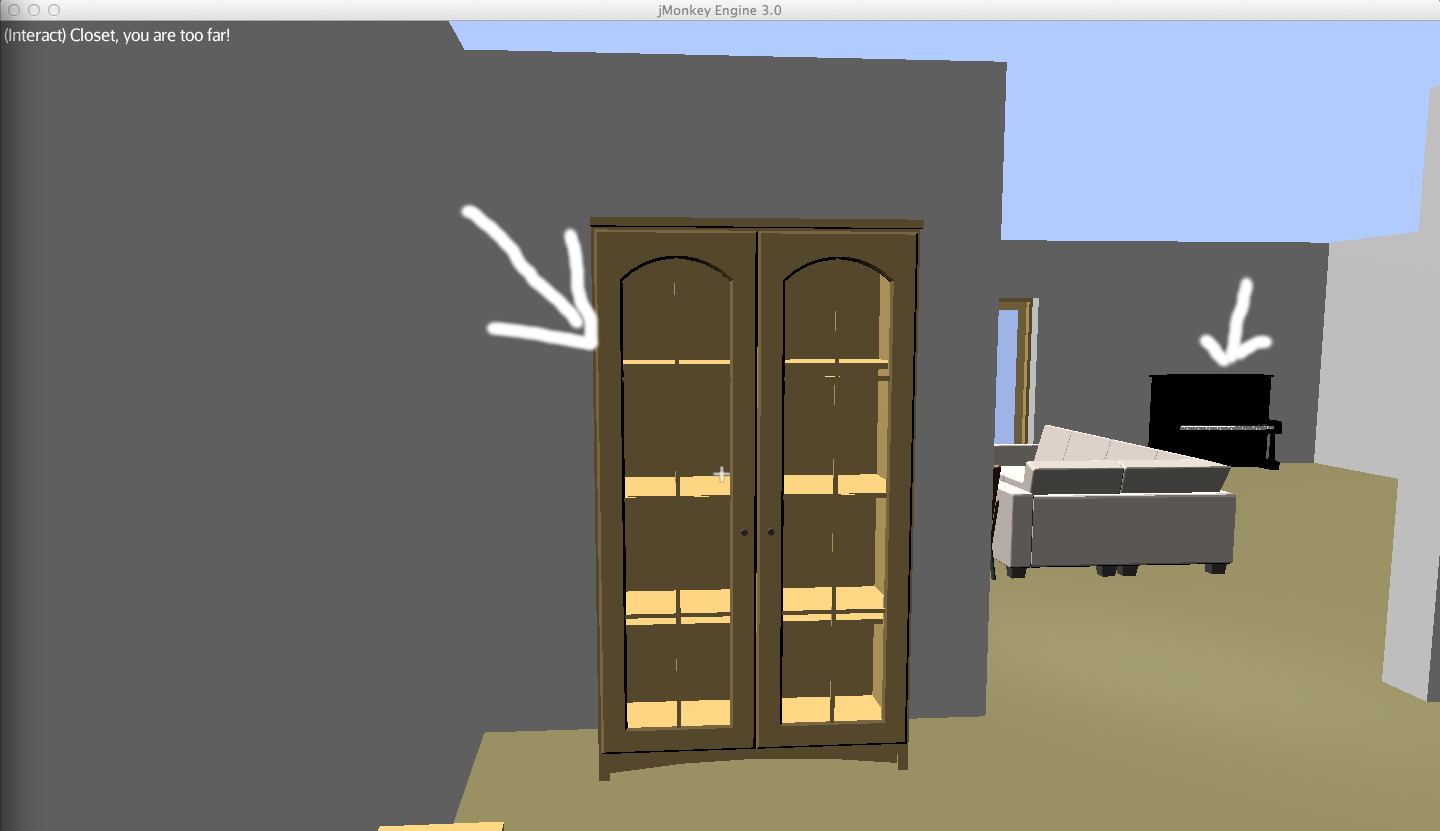
\includegraphics[width=0.4\columnwidth]{gfx/Chapter_EvaluationScenarios/bedroom}
%         \label{fig:eval_alf_bedroom}
%     }
%     \subfig[]{
%         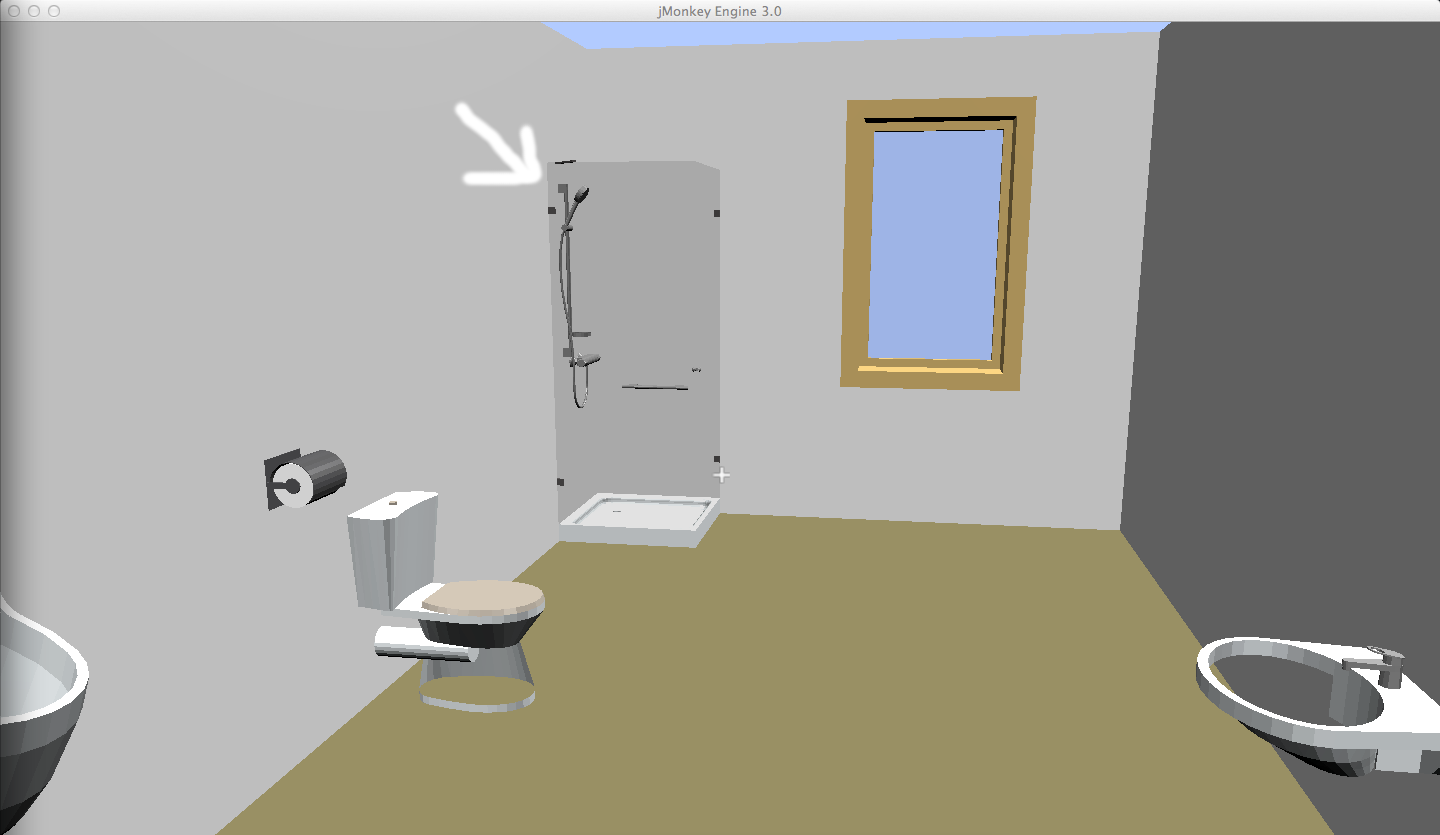
\includegraphics[width=0.4\columnwidth]{gfx/Chapter_EvaluationScenarios/bathroom}
%         \label{fig:eval_alf_bathroom}
%     }
%     \subfig[]{
%         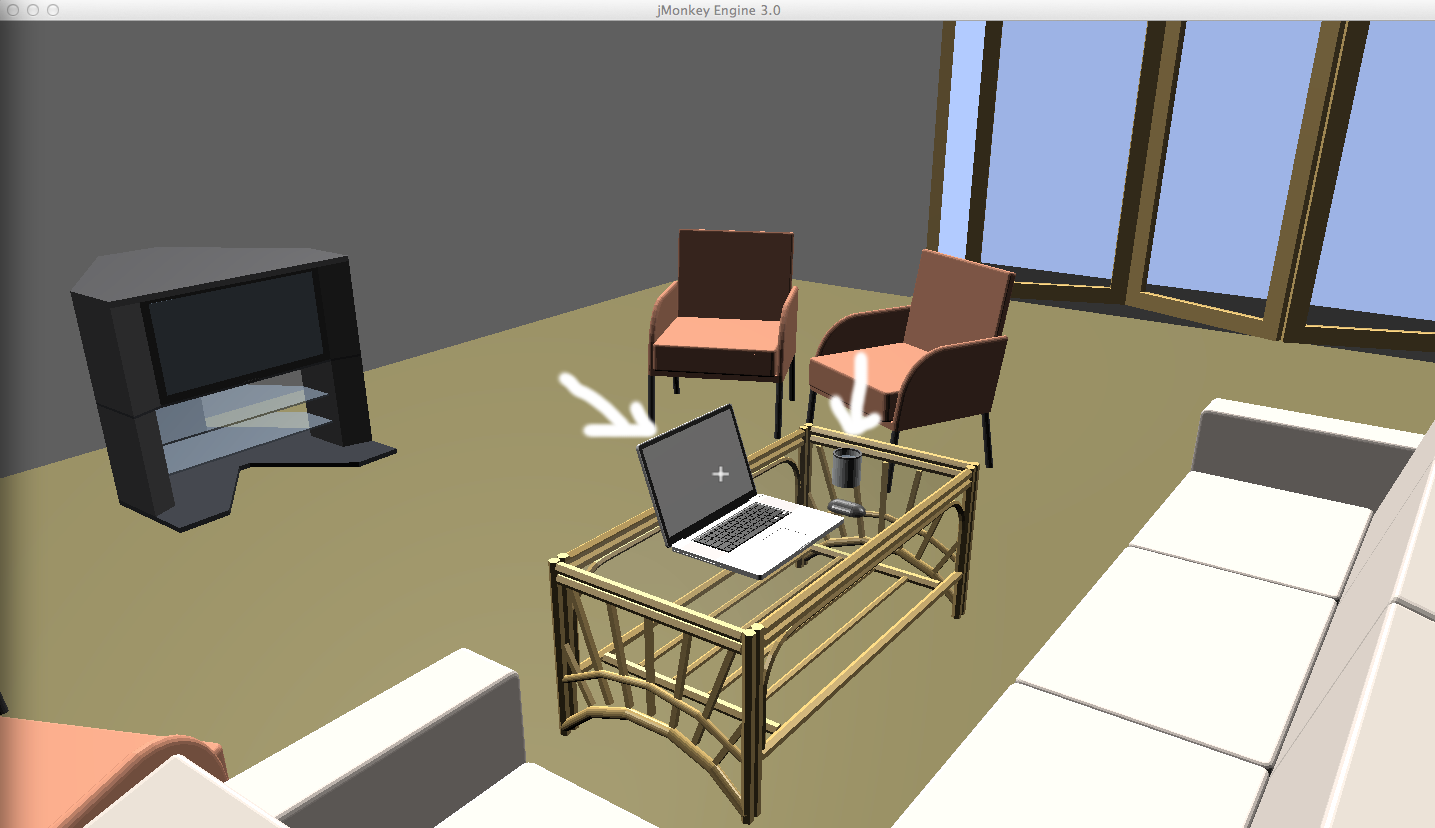
\includegraphics[width=0.4\columnwidth]{gfx/Chapter_EvaluationScenarios/living}
%         \label{fig:eval_alf_living}
%     }
%     \subfig[]{
%         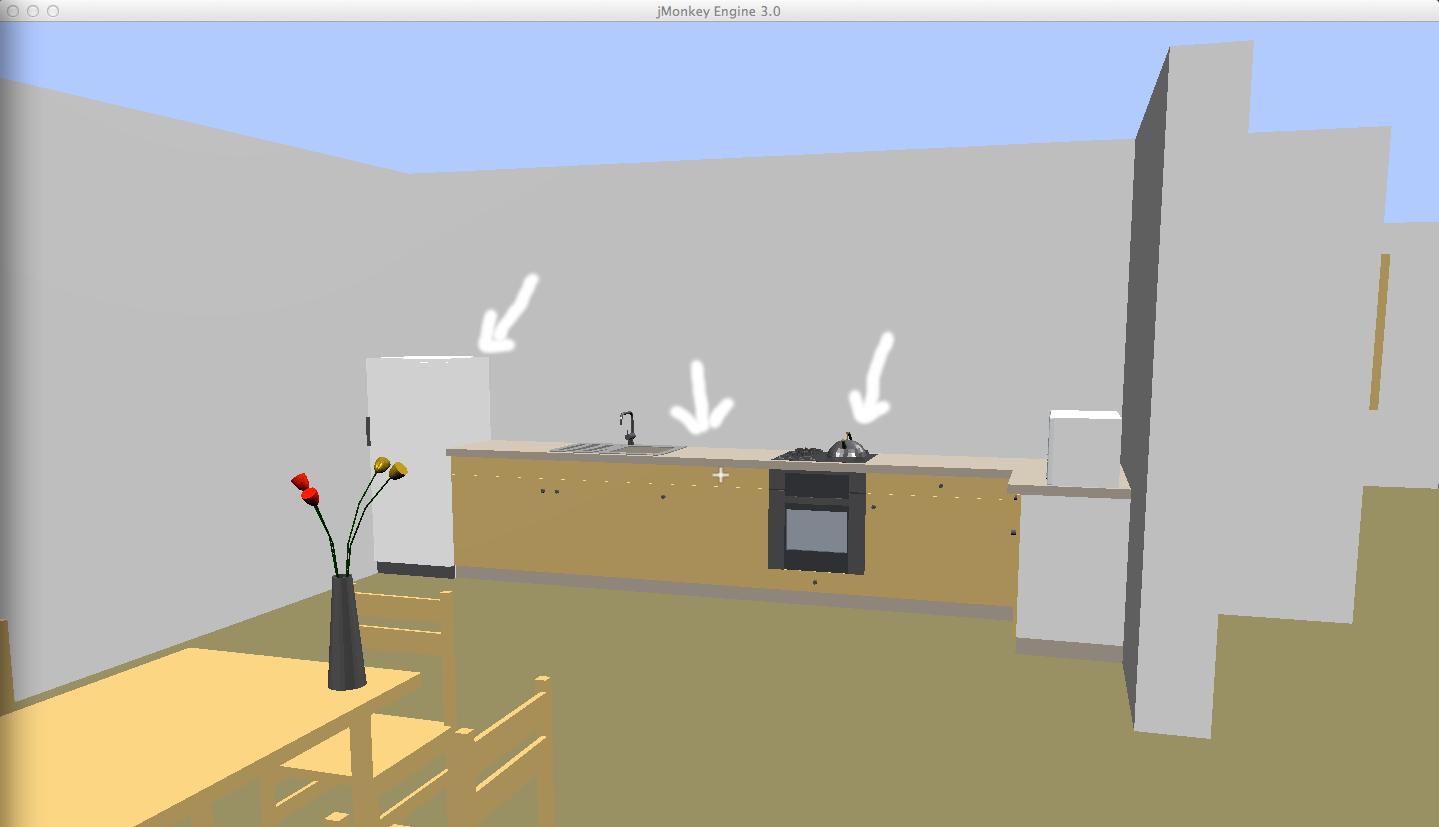
\includegraphics[width=0.4\columnwidth]{gfx/Chapter_EvaluationScenarios/kitchen}
%         \label{fig:eval_alf_kitchen}
%     }    
%     \caption{Screenshots of the running ALF simulation, highlighting objects the simulation user can interact with.}
%     \label{fig:eval_alf_interactive}
% \end{figure}

\begin{figure}[h]
	\begin{center}
		$
			\begin{array}{cc}
				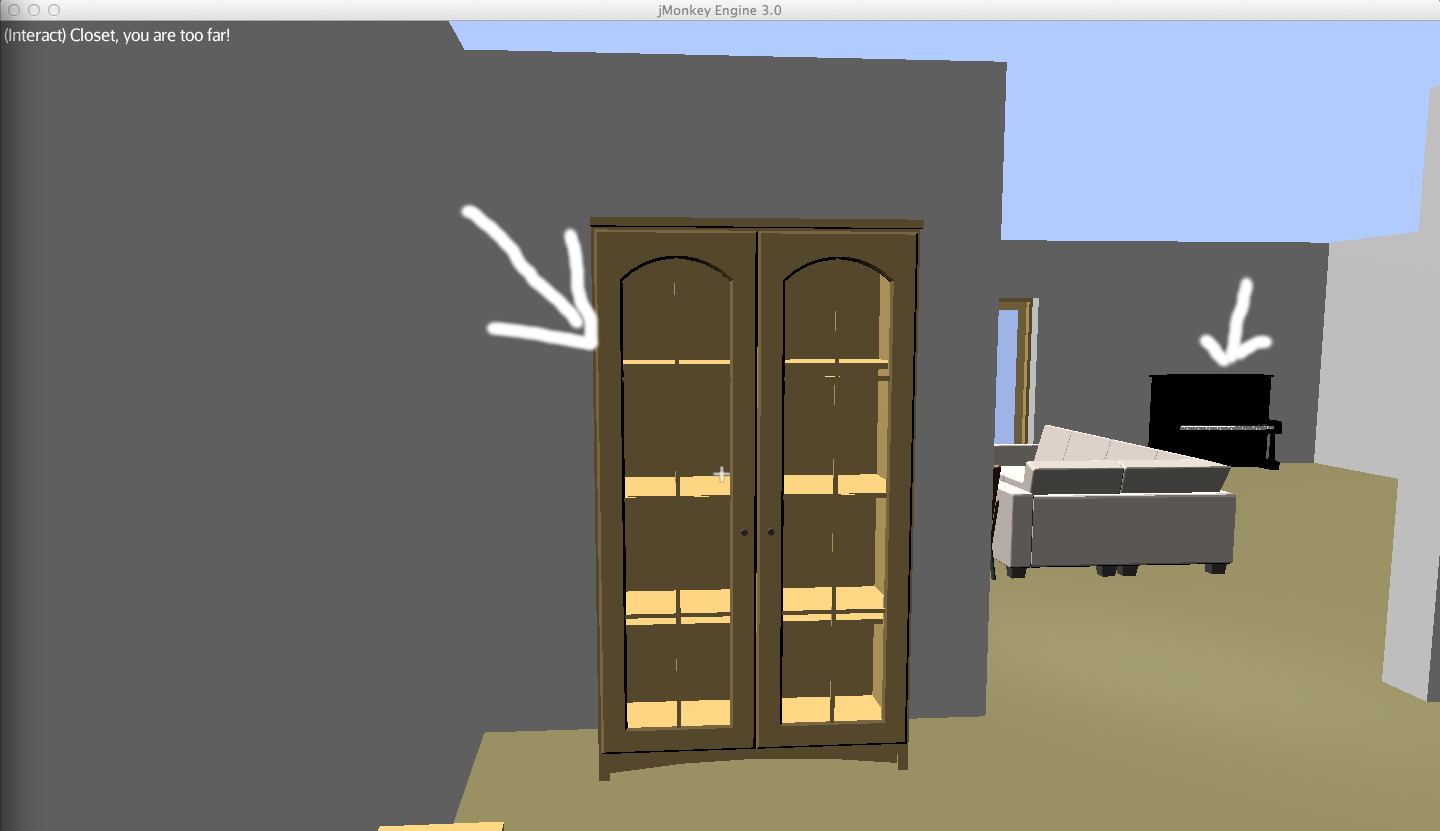
\includegraphics[width=0.45\columnwidth]{gfx/Chapter_EvaluationScenarios/bedroom}&
				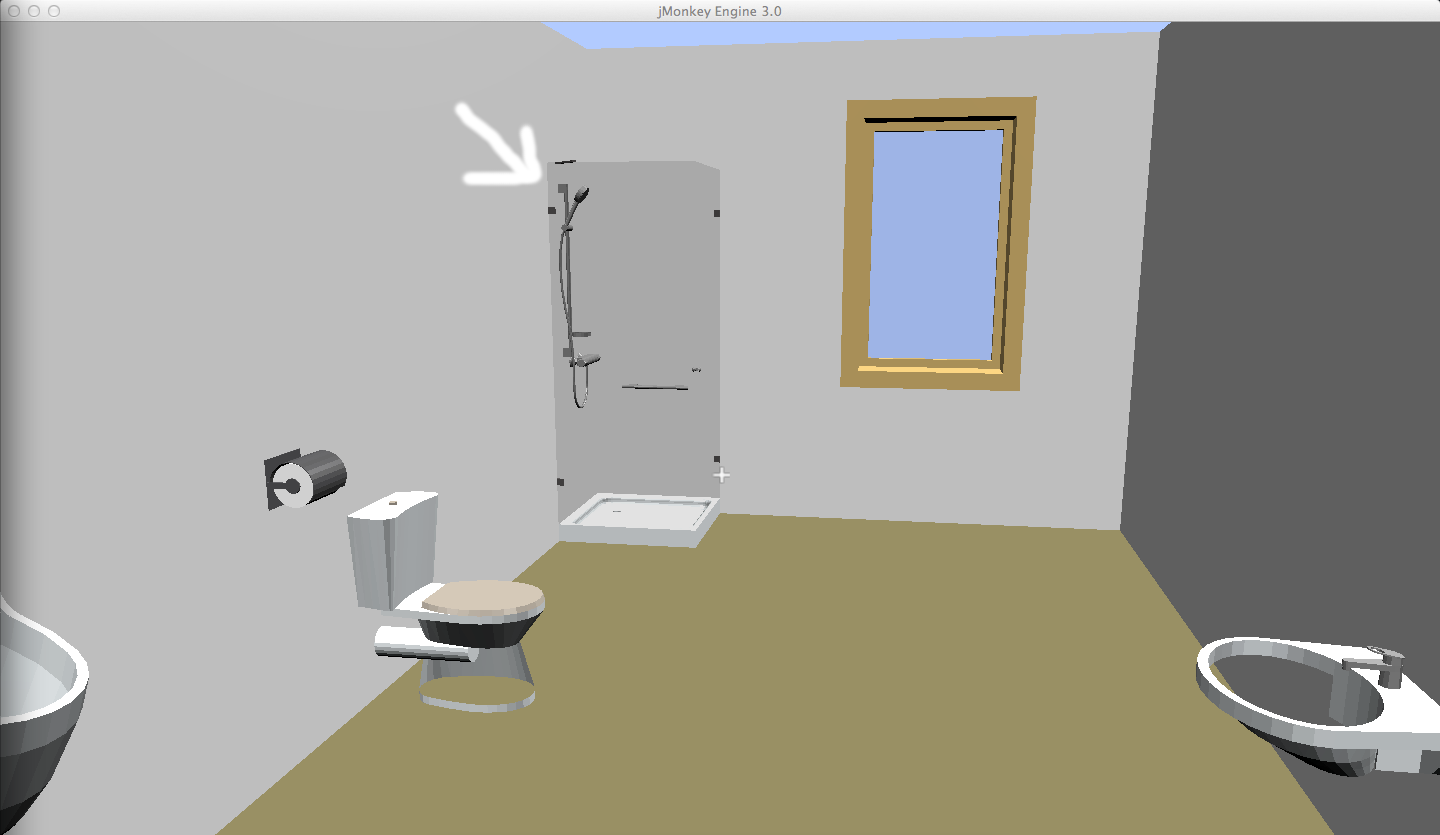
\includegraphics[width=0.45\columnwidth]{gfx/Chapter_EvaluationScenarios/bathroom}
			\end{array}
		$
		$
			\begin{array}{cc}
				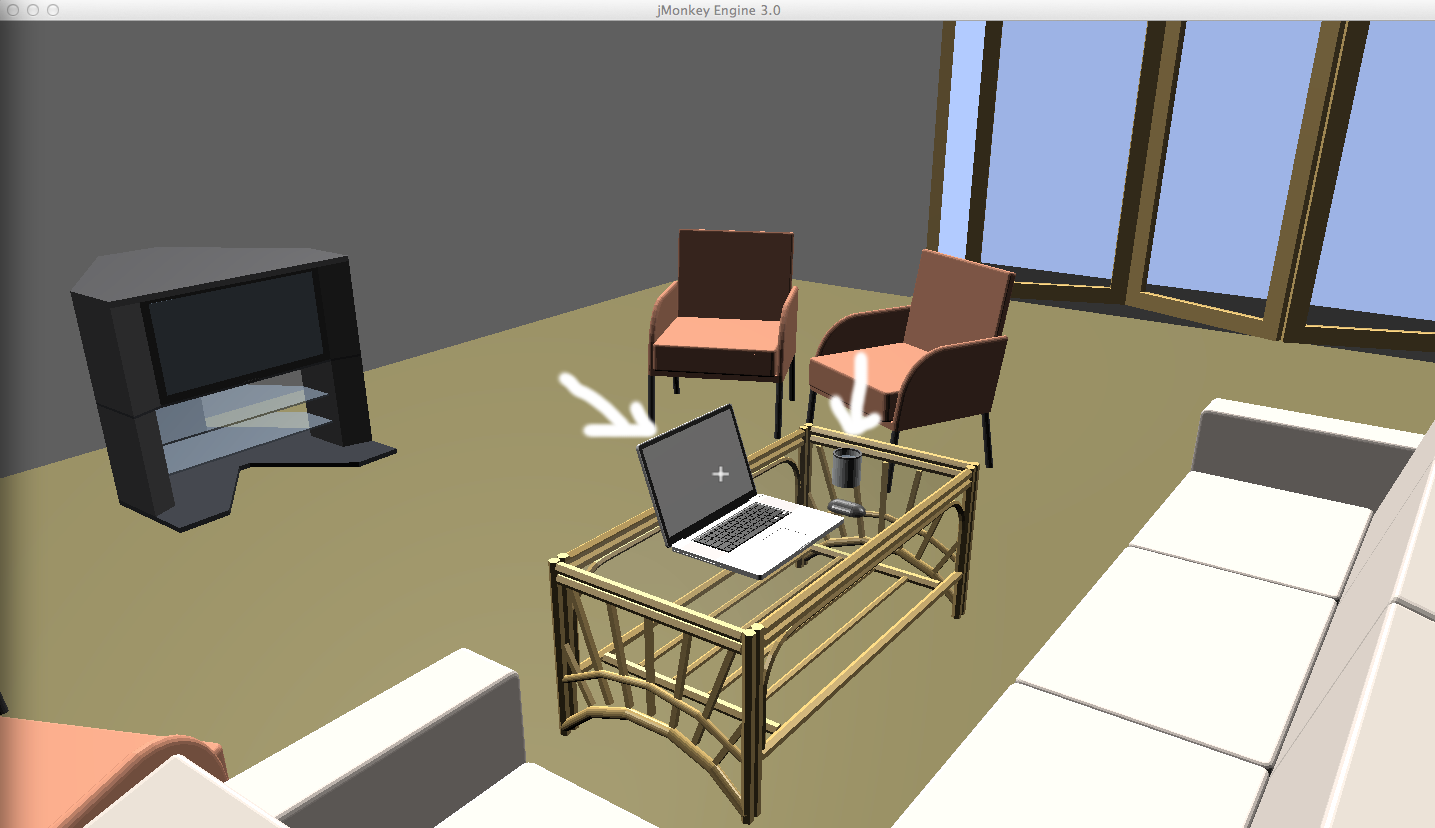
\includegraphics[width=0.45\columnwidth]{gfx/Chapter_EvaluationScenarios/living}&
				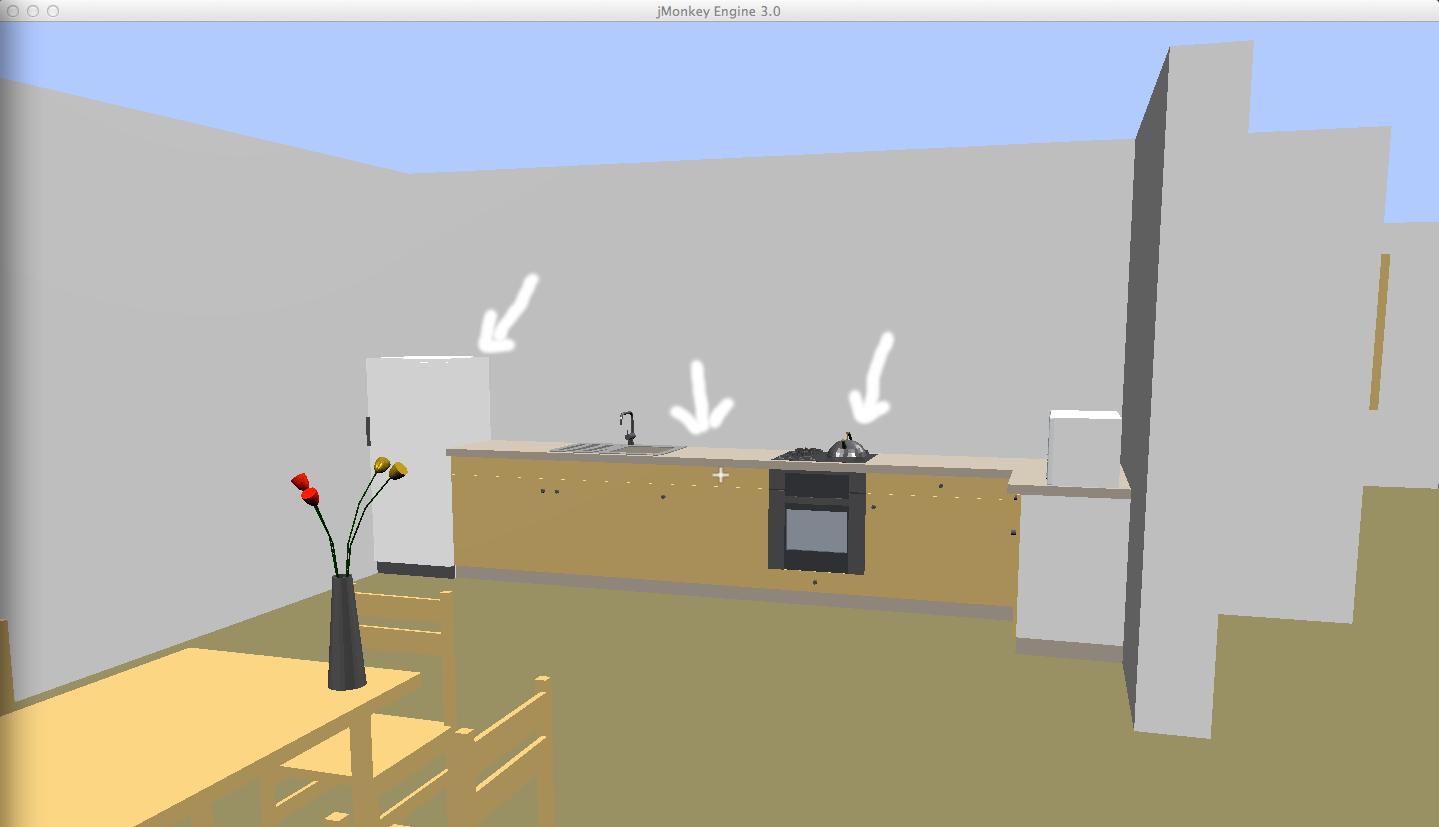
\includegraphics[width=0.45\columnwidth]{gfx/Chapter_EvaluationScenarios/kitchen}
			\end{array}
		$
	\end{center}
	\caption{Screenshots of the running Assisted Living Facility simulation, highlighting objects the simulation user can interact with.}
	\label{fig:eval_alf_interactive}
\end{figure}

The story unfolds with the following steps:
\begin{enumerate}
	\item You wake up in your bedroom. You just got off your bed; now walk towards the Closet in your bedroom. If you get close enough, the Closet will be added to the ActionSpace. Take note of this in the ContextClient. At this point, the ADL Service should ask the resided if she/he needs assistance with ''getting dressed''.
	\item Next, got into the bathroom. Approach the Shower, when close enough, it will be in the ActionSpace. Again, the ADL Service would detect a highly possible activity and would asks the resident if she/he needs assistance with ''takings a shower''.
	\item Go to the living room, pick up the cup and go to the kitchen. Place it near the Stove (on the Sink counter-top), pick up the coffee Pot and try pouring coffee into the cup. This kind of action is not implemented visually (pouring coffee), but you will see that the system knows exactly what you are doing (if the volume of your computer is turned one, you might be able to hear the audio feedback as well)! You will notice that the series of actions in this step are possible only if the items you are interacting with are in the ActionSpace.
	\item Approach the Fridge. When close enough, it will be in the ActionSpace. The ADL Service would ask the resident if she/he needs assistance feeding.
	\item Try interacting with the laptop to read your email (if the volume of your computer is turned one, you might be able to hear the audio feedback as well). The action is not visually implemented, you will get a system message instead!
	\item As a last step, walk around the apartment and observe how various objects get categorized, added/removed from SSM sets, as they enter/leave the view sight oh the agent, and as the agent gets closer/further from them.
\end{enumerate}

There's an easter egg hidden somewhere around, have you found it? If no, then try interacting with the piano. Interact with it a few times :).\\

When you arrive to this point, you have successfully performed the task.
% section eval_alf_scenario (end)
%************************************************
\section{Scenario 3: Childproof} % (fold)
\label{sec:eval_childproof_scenario}
%************************************************
The hypothetical problem we are facing as part of this task is that families cannot make their homes secure enough for their children. To provide a solution for this problem, there's a need for a system to constantly monitoring the objects a child should keep away from and should not be interacting with. Based on this context information, we can further build various software service to secure the house from the child's actions. One example of such service is the ''Secure Outlets Service'' (SOS). This service has to detect whenever a child is approaching an outlet with a small object, in which case it should shut down the electricity switch for outlets, preventing the child from the possibly of getting electrocuted.\\

For this task, please imagine yourself as being the researcher in charge to develop this system. Once again, you decide to design your system based on the egocentric interaction paradigm, as it can categorizes all the objects of interest around the human agent. In order to validate your design, you decide to simulate the system first.\\

In this exercise, you will be provided with the virtual model of the simulated environment in the Blender\footnote{\url{http://www.blender.org/}} format. Blender is a free and open-source software for creating 3D virtual models, animations and more.\\

Using the EgoSim framework, you will augment this model to monitor the objects required by your system. Afterwards, based on the frameworks API, you will write the condition for the SOS to shut the electricity down in the outlets.\\

A recording of sequentially executing the steps in this scenario is available; see Appendix \ref{ch:videos}.\\

Next, please follow the steps in the User Guide \ref{ch:user_guide} to set up a new simulation.\\

After you have successfully set up and ran the simulation, as part of the interactions you do with the environment, pick up the Pen from the table and move with it close to one of the outlets, so that the Outlet is in the ActionSpace. When you arrive to this point, you have successfully performed the task.\\
% section eval_childproof_scenario (end)